\documentclass[11pt, aspectratio=169]{beamer}

% Gọi file cấu hình chung
\usepackage{./common_style}
\usepackage{tikz} % Thêm thư viện để vẽ hình
\usetikzlibrary{arrows.meta} % Thư viện để tùy chỉnh mũi tên

\title[PT ĐƯỜNG THẲNG (LINEAR EQUATION)]{PT ĐƯỜNG THẲNG (LINEAR EQUATION)}

\author[Trần Đức Mạnh]{
    Trần Đức Mạnh \\[0.2cm] 
    \today \\[0.4cm] 
    
\includegraphics[width=0.3\textwidth]{"/home/trandmanh/Projects/Funix/images/linearequation.png"}
} 

\titlegraphic{}

\begin{document}

% ==================== TRANG BÌA ====================
\begin{frame}
    \titlepage
\end{frame}

\section{Vector pháp tuyến và vector chỉ phương}

\subsection{Vector pháp tuyến}

\begin{frame}[fragile]
    \frametitle{\thesection. \insertsection}
    \framesubtitle{\thesection.\thesubsection. Vector pháp tuyến (Normal vector) của đường thẳng}
    \vspace{-0.5cm}
    \begin{columns}[T, onlytextwidth]
        \begin{column}{0.48\textwidth}
            \begin{block}{Định nghĩa}
                \footnotesize
                Vector $\vec{n} \neq \vec{0}$ được gọi là \textbf{vector pháp tuyến} của đường thẳng $\Delta$ nếu giá của $\vec{n}$ \textbf{vuông góc} với $\Delta$.
            \end{block}
            
            
            \begin{block}{Tính chất}
                \footnotesize
                \begin{itemize}
                    \item Nếu $\vec{n}$ là vector pháp tuyến của $\Delta$ thì mọi vector $k\vec{n}\;(k \neq 0)$ cũng là vector pháp tuyến của $\Delta$.
                    \item Một đường thẳng có \textbf{vô số} vector pháp tuyến, tất cả đều cùng phương với nhau.
                    \item Vector pháp tuyến \textbf{không xác định} phương của đường thẳng (chỉ xác định hướng vuông góc).
                \end{itemize}
            \end{block}
        \end{column}
        
        \begin{column}{0.48\textwidth}
            \centering
            \begin{tikzpicture}[>=Stealth, thick, scale=0.8, every node/.style={scale=0.85}]
                % Trục tọa độ 
                \draw[->, gray!60, thin] (-0.5,0) -- (5.5,0) node[right, text=black] {$x$};
                \draw[->, gray!60, thin] (0,-0.5) -- (0,5.5) node[above, text=black] {$y$};
                
                % Đường thẳng Delta
                \draw[black, ultra thick] (-0.2,-0.2) -- (5.2,5.2) node[right] {$\Delta$};
                
                % Các điểm gốc M trên đường thẳng Delta
                \coordinate (M1) at (1.2,1.2);
                \coordinate (M2) at (2.5,2.5);
                \coordinate (M3) at (3.8,3.8);
                \coordinate (M4) at (0.5,0.5);
                
                % Các vector pháp tuyến (Chữ nằm ở đỉnh mũi tên, không bị đè)
                \draw[->, blue, ultra thick] (M1) -- ++(-1.2,1.2) node[above left] {$\vec{n}_1$};
                \draw[->, red, thick] (M2) -- ++(1,-1) node[below right] {$\vec{n}_2$};
                \draw[->, green!60!black, thick] (M3) -- ++(-1.5,1.5) node[above left] {$\vec{n}_3$};
                \draw[->, orange, thick] (M4) -- ++(0.7,-0.7) node[below right] {$\vec{n}_4$};
                
                % Ký hiệu vuông góc 
                \draw[gray, thin] ($(M1)+(0.25,0.25)$) -- ++(-0.25,0.25) -- ++(-0.25,-0.25);
                \draw[gray, thin] ($(M2)+(0.25,0.25)$) -- ++(0.25,-0.25) -- ++(-0.25,-0.25);
                \draw[gray, thin] ($(M3)+(-0.25,-0.25)$) -- ++(-0.25,0.25) -- ++(0.25,0.25);
                \draw[gray, thin] ($(M4)+(-0.25,-0.25)$) -- ++(0.25,-0.25) -- ++(0.25,0.25);
                
                % Dấu chấm tại các điểm gốc
                \filldraw[black] (M1) circle (1.2pt);
                \filldraw[black] (M2) circle (1.2pt);
                \filldraw[black] (M3) circle (1.2pt);
                \filldraw[black] (M4) circle (1.2pt);
            \end{tikzpicture}
            
            \vspace{0.4cm}
            
            % Phần nhận xét được gộp chung và căn lề để không bị tràn chữ
            \begin{minipage}{0.9\textwidth}
                \footnotesize
                \textbf{Nhận xét:} $\vec{n}_1, \vec{n}_2, \vec{n}_3, \vec{n}_4$ là các vector pháp tuyến của $\Delta$, chúng đều cùng phương với nhau.
            \end{minipage}
        \end{column}
    \end{columns}
\end{frame}


\begin{frame}[fragile]
    \frametitle{\thesection. \insertsection}
    \framesubtitle{\thesection.2. Vector chỉ phương (Direction vector) của đường thẳng}
    \vspace{-0.5cm}
    \begin{columns}[T, onlytextwidth]
        \begin{column}{0.48\textwidth}
            \begin{block}{Định nghĩa}
                \footnotesize
                Vector $\vec{u} \neq \vec{0}$ được gọi là \textbf{vector chỉ phương} của đường thẳng $\Delta$ nếu giá của $\vec{u}$ \textbf{song song} hoặc \textbf{trùng} với $\Delta$.
            \end{block}
            
            \vspace{0.1cm}
            
            \begin{block}{Tính chất}
                \footnotesize
                \begin{itemize}
                    \item Nếu $\vec{u}$ là vector chỉ phương của $\Delta$ thì mọi vector $k\vec{u}\;(k \neq 0)$ cũng là vector chỉ phương của $\Delta$.
                    \item Một đường thẳng có \textbf{vô số} vector chỉ phương, tất cả đều cùng phương với nhau.
                    \item Vector chỉ phương và vector pháp tuyến của cùng một đường thẳng luôn \textbf{vuông góc} với nhau ($\vec{u} \cdot \vec{n} = 0$).
                \end{itemize}
            \end{block}
        \end{column}
        

        \begin{column}{0.48\textwidth}
            \centering
            % Đã giảm scale xuống 0.75 để vừa vặn với slide
            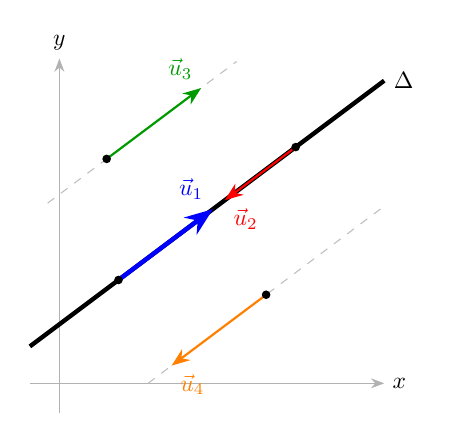
\begin{tikzpicture}[>=Stealth, thick, scale=0.75, every node/.style={scale=0.85}]
                % Trục tọa độ
                \draw[->, gray!60, thin] (-0.5,0) -- (5.5,0) node[right, text=black] {$x$};
                \draw[->, gray!60, thin] (0,-0.5) -- (0,5.5) node[above, text=black] {$y$};
                
                % Đường thẳng Delta
                \draw[black, ultra thick] (-0.5, 0.625) -- (5.5, 5.125) node[right] {$\Delta$};
                
                % --- CÁC VECTOR NẰM TRÊN ĐƯỜNG THẲNG ---
                \coordinate (M1) at (1, 1.75);
                \coordinate (M2) at (4, 4);
                
                % u1 (hướng lên trên)
                \draw[->, blue, ultra thick] (M1) -- ++(1.6, 1.2) node[above left] {$\vec{u}_1$};
                % u2 (hướng xuống dưới)
                \draw[->, red, thick] (M2) -- ++(-1.2, -0.9) node[below right] {$\vec{u}_2$};
                
                % Dấu chấm gốc trên đường thẳng
                \filldraw[black] (M1) circle (1.5pt);
                \filldraw[black] (M2) circle (1.5pt);
                
                % --- CÁC VECTOR SONG SONG ---
                \coordinate (M3) at (0.8, 3.8); 
                \coordinate (M4) at (3.5, 1.5); 
                
                % Giá của u3 và u4 (đường nét đứt mờ)
                \draw[dashed, gray!50, thin] (-0.2, 3.05) -- (3, 5.45);
                \draw[dashed, gray!50, thin] (1.5, 0) -- (5.5, 3);
                
                % u3 (hướng lên trên, song song)
                \draw[->, green!60!black, thick] (M3) -- ++(1.6, 1.2) node[above left] {$\vec{u}_3$};
                % u4 (hướng xuống dưới, song song)
                \draw[->, orange, thick] (M4) -- ++(-1.6, -1.2) node[below right] {$\vec{u}_4$};
                
                % Dấu chấm gốc của các vector song song
                \filldraw[black] (M3) circle (1.5pt);
                \filldraw[black] (M4) circle (1.5pt);
                
            \end{tikzpicture}
            
            \vspace{0.15cm} % Giảm khoảng cách để chống tràn
            
            % Nhận xét
            \begin{minipage}{0.95\textwidth}
                \footnotesize
                \textbf{Nhận xét:} $\vec{u}_1, \vec{u}_2, \vec{u}_3, \vec{u}_4$ là các vector chỉ phương của $\Delta$, chúng có giá song song hoặc trùng nhau (cùng phương).
            \end{minipage}
        \end{column}
    \end{columns}
\end{frame}


\section{Phương trình đường thẳng trong mặt phẳng Oxy}

\subsection{Phương trình tổng quát}

\begin{frame}[fragile]
    \frametitle{\thesection. \insertsection}
    \framesubtitle{\thesection.\thesubsection. Dạng tổng quát (General form)}
    \vspace{-0.5cm}

    \begin{columns}[T, onlytextwidth]
        \begin{column}{0.48\textwidth}
            \begin{block}{Định nghĩa}
                \footnotesize
                Trong mặt phẳng $Oxy$, cho đường thẳng $\Delta$ đi qua $M(x_0; y_0)$ và có vector pháp tuyến $\vec{n} = (A; B) \neq \vec{0}$.
                
                Với mọi điểm $N(x; y)$ bất kỳ thuộc $\Delta$, ta luôn có:
                \[
                    \vec{n} \cdot \overrightarrow{MN} = 0
                \]
                \[
                    \Leftrightarrow A(x - x_0) + B(y - y_0) = 0
                \]
                \[
                    \Leftrightarrow Ax + By - (Ax_0 + By_0) = 0
                \]
                Đặt $C = -(Ax_0 + By_0)$, ta được phương trình:
                \[
                    \boxed{Ax + By + C = 0} \quad (A^2 + B^2 \neq 0)
                \]
                Đây gọi là \textbf{phương trình tổng quát} của đường thẳng $\Delta$.
            \end{block}
        \end{column}
        
        \begin{column}{0.48\textwidth}
            \centering
            \vspace{0.4cm} % Đẩy đồ thị xuống một chút để cân bằng với khối text bên trái
            \begin{tikzpicture}[>=Stealth, thick, scale=0.85, every node/.style={scale=0.9}]
                % Trục tọa độ
                \draw[->, gray!60, thin] (-0.5,0) -- (6.5,0) node[right, text=black] {$x$};
                \draw[->, gray!60, thin] (0,-1.0) -- (0,5.5) node[above, text=black] {$y$};
                
                % Đường thẳng Delta 
                \draw[blue, ultra thick] (-0.5, 3.375) -- (5.5, -1.125) node[right, text=blue] {$\Delta$};
                
                % Điểm M và N
                \coordinate (M) at (1.2, 2.1);
                \coordinate (N) at (4.4, -0.3);
                
                % Vector MN (màu cam, dời text xuống dưới để không đè vào góc vuông)
                \draw[->, orange, thick] (M) -- (N) node[midway, below=0.15cm, sloped] {$\overrightarrow{MN}$};
                
                % Điểm và nhãn (Đặt nhãn khéo léo để không cắt vào đường thẳng)
                \filldraw[black] (M) circle (1.5pt) node[below left] {$M(x_0; y_0)$};
                \filldraw[black] (N) circle (1.5pt) node[below right] {$N(x; y)$};
                
                % Vector pháp tuyến n xuất phát thẳng từ M để chứng minh tính vuông góc rõ rệt
                \coordinate (N_tip) at ($(M) + (1.5, 2)$);
                \draw[->, red, ultra thick] (M) -- (N_tip) node[above left] {$\vec{n} = (A; B)$};
                
                % Ký hiệu vuông góc tự động tính toán chuẩn xác bằng thư viện calc
                \coordinate (U) at ($(M)!3.5mm!(N)$);
                \coordinate (V) at ($(M)!3.5mm!(N_tip)$);
                \coordinate (W) at ($(U)+(V)-(M)$);
                \draw[gray, thin] (U) -- (W) -- (V);
                
                % Chú thích trực quan
                \node[gray, right] at ($(M) + (0.8, 0.9)$) {$\vec{n} \perp \overrightarrow{MN}$};
            \end{tikzpicture}
        \end{column}
    \end{columns}
\end{frame}


\subsection{Phương trình tham số}

\begin{frame}[fragile]
    \frametitle{\thesection. \insertsection}
    \framesubtitle{\thesection.\thesubsection. Phương trình tham số (Parametric equation)}
    \vspace{-0.5cm}
    \begin{columns}[T, onlytextwidth]
        \begin{column}{0.48\textwidth}
            \begin{block}{Định nghĩa}
                \footnotesize
                Trong mặt phẳng $Oxy$, cho đường thẳng $\Delta$ đi qua điểm $M(x_0; y_0)$ và có vector chỉ phương $\vec{u} = (u_1; u_2) \neq \vec{0}$.
                
                Với mọi điểm $N(x; y)$ bất kỳ thuộc $\Delta$, ta luôn có vector $\overrightarrow{MN}$ cùng phương với vector $\vec{u}$.
                
                Do đó, tồn tại một số thực $t$ sao cho:
                \[
                    \overrightarrow{MN} = t\vec{u} \Leftrightarrow
                    \begin{cases}
                        x - x_0 = tu_1 \\
                        y - y_0 = tu_2
                    \end{cases}
                \]
                Hay viết lại thành \textbf{phương trình tham số} của $\Delta$:
                \[
                    \boxed{
                    \begin{cases}
                        x = x_0 + tu_1 \\
                        y = y_0 + tu_2
                    \end{cases}
                    } \quad (t \in \mathbb{R})
                \]
            \end{block}
        \end{column}
        
        \begin{column}{0.48\textwidth}
            \centering
            \vspace{0.2cm} % Giảm khoảng cách để chống tràn
            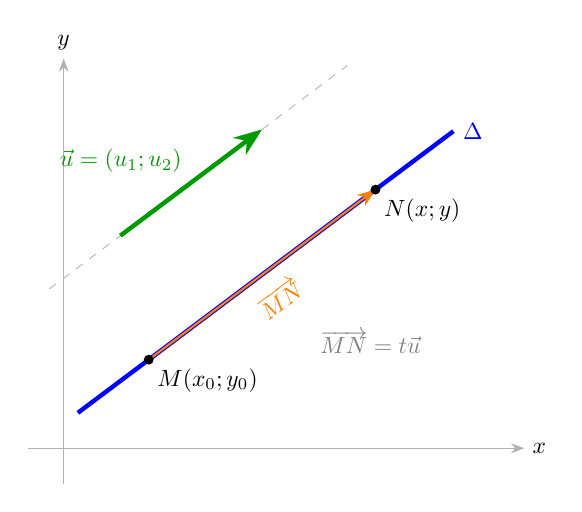
\begin{tikzpicture}[>=Stealth, thick, scale=0.9, every node/.style={scale=0.85}]
                % Trục tọa độ
                \draw[->, gray!60, thin] (-0.5,0) -- (6.5,0) node[right, text=black] {$x$};
                \draw[->, gray!60, thin] (0,-0.5) -- (0,5.5) node[above, text=black] {$y$};
                
                % Đường thẳng Delta
                \draw[blue, ultra thick] (0.2, 0.5) -- (5.5, 4.475) node[right, text=blue] {$\Delta$};
                
                % Điểm M cố định và N bất kỳ trên Delta
                \coordinate (M) at (1.2, 1.25);
                \coordinate (N) at (4.4, 3.65);
                
                % Vector MN (màu cam)
                \draw[->, orange, thick] (M) -- (N) node[midway, below=0.15cm, sloped] {$\overrightarrow{MN}$};
                
                % Các điểm và nhãn
                \filldraw[black] (M) circle (1.5pt) node[below right] {$M(x_0; y_0)$};
                \filldraw[black] (N) circle (1.5pt) node[below right] {$N(x; y)$};
                
                % Vector chỉ phương u (màu xanh lá, vẽ song song bên ngoài để dễ nhìn)
                \coordinate (U_start) at (0.8, 3.0);
                \coordinate (U_end) at (2.8, 4.5);
                
                % Giá của u (nét đứt)
                \draw[dashed, gray!50, thin] (-0.2, 2.25) -- (4, 5.4);
                
                \draw[->, green!60!black, ultra thick] (U_start) -- (U_end) node[midway, above left] {$\vec{u} = (u_1; u_2)$};
                
                % Chú thích trực quan quan hệ giữa 2 vector
                \node[gray, right] at (3.5, 1.5) {$\overrightarrow{MN} = t\vec{u}$};
            \end{tikzpicture}
        \end{column}
    \end{columns}
\end{frame}



\subsection{Phương trình chính tắc}

\begin{frame}[fragile]
    \frametitle{\thesection. \insertsection}
    \framesubtitle{\thesection.\thesubsection. Phương trình chính tắc (Canonical equation)}
    \vspace{-0.5cm}
    \begin{columns}[T, onlytextwidth]
        \begin{column}{0.48\textwidth}
            \begin{block}{Định nghĩa}
                \footnotesize
                Từ hệ phương trình tham số của $\Delta$ đi qua $M(x_0; y_0)$ với vector chỉ phương $\vec{u} = (u_1; u_2)$:
                
                \centering $\begin{cases} x = x_0 + tu_1 \\ y = y_0 + tu_2 \end{cases}$
                \flushleft
                
                Nếu $u_1 \neq 0$ và $u_2 \neq 0$, ta rút $t$ từ hệ trên được:
                
                \centering $t = \frac{x - x_0}{u_1}$ \quad và \quad $t = \frac{y - y_0}{u_2}$
                \flushleft
                
                Cho hai biểu thức bằng nhau, ta được \textbf{phương trình chính tắc} của $\Delta$:
                \[
                    \boxed{ \frac{x - x_0}{u_1} = \frac{y - y_0}{u_2} }
                \]
            \end{block}
            

            \footnotesize
            \textbf{* Lưu ý:} Nếu $u_1 = 0$ hoặc $u_2 = 0$, đường thẳng $\Delta$ \textbf{không có} phương trình chính tắc.
        \end{column}
        
        \begin{column}{0.48\textwidth}
            \centering
            \vspace{0.1cm}
            \begin{tikzpicture}[>=Stealth, thick, scale=0.9, every node/.style={scale=0.85}]
                % Trục tọa độ
                \draw[->, gray!60, thin] (-0.5,0) -- (6.5,0) node[right, text=black] {$x$};
                \draw[->, gray!60, thin] (0,-0.5) -- (0,5.8) node[above, text=black] {$y$};
                
                % Đường thẳng Delta
                \draw[blue, ultra thick] (0.2, 1.0) -- (5.8, 5.2) node[right, text=blue] {$\Delta$};
                
                % Điểm M và N 
                \coordinate (M) at (1.2, 1.75);
                \coordinate (N) at (4.8, 4.45);
                
                % Tam giác lớn cho MN (nét đứt cam)
                \coordinate (P) at (4.8, 1.75);
                \draw[dashed, orange, thick] (M) -- (P) node[midway, below] {$x - x_0$};
                \draw[dashed, orange, thick] (P) -- (N) node[midway, right] {$y - y_0$};
                % Ký hiệu vuông góc tại P
                \draw[gray, thin] ($(P)+(-0.25,0)$) -- ++(0,0.25) -- ++(0.25,0);
                
                % Vector u và tam giác nhỏ (xanh lá)
                \coordinate (U) at (2.8, 2.95);
                \coordinate (R) at (1.2, 2.95);
                
                \draw[dashed, green!60!black, thick] (M) -- (R) node[midway, left] {$u_2$};
                \draw[dashed, green!60!black, thick] (R) -- (U) node[midway, above] {$u_1$};
                \draw[->, green!60!black, ultra thick] (M) -- (U) node[midway, below right] {$\vec{u}$};
                % Ký hiệu vuông góc tại R
                \draw[gray, thin] ($(R)+(0,-0.25)$) -- ++(0.25,0) -- ++(0,0.25);
                
                % Mũi tên cam MN đè lên một phần đường thẳng
                \draw[->, orange, thick] (M) -- (N);
                
                % Các điểm và nhãn (Đã dời M xuống góc dưới-phải để trống không gian)
                \filldraw[black] (M) circle (1.5pt) node[below] {$M(x_0; y_0)$};
                \filldraw[black] (N) circle (1.5pt) node[above left] {$N(x; y)$};
                
                
            \end{tikzpicture}
        \end{column}
    \end{columns}
\end{frame}



\subsection{Vị trí tương đối của hai đường thẳng}

\begin{frame}[fragile]
    \frametitle{\thesection. \insertsection}
    \framesubtitle{\thesection.\thesubsection. Vị trí tương đối và số nghiệm}

    \begin{block}{Hệ phương trình giao điểm}
        \footnotesize
        Cho $d_1: a_1x + b_1y + c_1 = 0$ và $d_2: a_2x + b_2y + c_2 = 0$. 
        Tọa độ điểm chung của $d_1$ và $d_2$ là nghiệm của hệ:
        \[\begin{cases} a_1x + b_1y = -c_1 \\ a_2x + b_2y = -c_2 \end{cases}\]
    \end{block}
    
    \vspace{0.2cm}
    
    \begin{center}
    \setlength{\tabcolsep}{8pt} % Giảm khoảng cách giữa các cột
    \begin{tabular}{c c c}
        % Hàng 1: Hình vẽ
        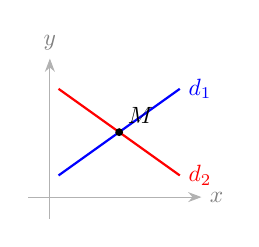
\begin{tikzpicture}[>=Stealth, thick, scale=0.55, every node/.style={scale=0.85}]
            \draw[->, gray!60, thin] (-0.5,0) -- (3.5,0) node[right, gray] {$x$};
            \draw[->, gray!60, thin] (0,-0.5) -- (0,3.2) node[above, gray] {$y$};
            \draw[blue, thick] (0.2, 0.5) -- (3.0, 2.5) node[right, blue] {$d_1$};
            \draw[red, thick] (0.2, 2.5) -- (3.0, 0.5) node[right, red] {$d_2$};
            \filldraw[black] (1.6, 1.5) circle (1.8pt) node[above right] {$M$};
        \end{tikzpicture}
        & 
        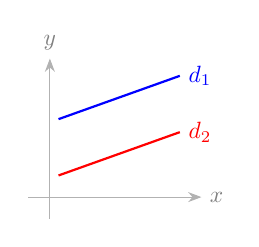
\begin{tikzpicture}[>=Stealth, thick, scale=0.55, every node/.style={scale=0.85}]
            \draw[->, gray!60, thin] (-0.5,0) -- (3.5,0) node[right, gray] {$x$};
            \draw[->, gray!60, thin] (0,-0.5) -- (0,3.2) node[above, gray] {$y$};
            \draw[blue, thick] (0.2, 1.8) -- (3.0, 2.8) node[right, blue] {$d_1$};
            \draw[red, thick] (0.2, 0.5) -- (3.0, 1.5) node[right, red] {$d_2$};
        \end{tikzpicture}
        & 
        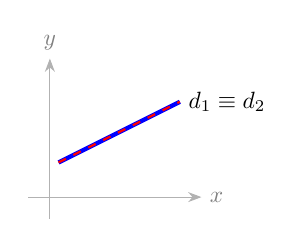
\begin{tikzpicture}[>=Stealth, thick, scale=0.55, every node/.style={scale=0.85}]
            \draw[->, gray!60, thin] (-0.5,0) -- (3.5,0) node[right, gray] {$x$};
            \draw[->, gray!60, thin] (0,-0.5) -- (0,3.2) node[above, gray] {$y$};
            \draw[blue, ultra thick] (0.2, 0.8) -- (3.0, 2.2);
            \draw[red, dashed, thick] (0.2, 0.8) -- (3.0, 2.2);
            \node[right, black] at (3.0, 2.2) {$d_1 \equiv d_2$};
        \end{tikzpicture}
        \\
        % Hàng 2: Chú thích với cỡ chữ tiny
        \begin{minipage}{0.25\textwidth}
            \centering
            \tiny
            \textbf{Cắt nhau} \\
            $1$ nghiệm duy nhất \\
            $\dfrac{a_1}{a_2} \neq \dfrac{b_1}{b_2}$
        \end{minipage}
        & 
        \begin{minipage}{0.25\textwidth}
            \centering
            \tiny
            \textbf{Song song} \\
            Vô nghiệm \\
            $\dfrac{a_1}{a_2} = \dfrac{b_1}{b_2} \neq \dfrac{c_1}{c_2}$
        \end{minipage}
        & 
        \begin{minipage}{0.25\textwidth}
            \centering
            \tiny
            \textbf{Trùng nhau} \\
            Vô số nghiệm \\
            $\dfrac{a_1}{a_2} = \dfrac{b_1}{b_2} = \dfrac{c_1}{c_2}$
        \end{minipage}
    \end{tabular}
    \end{center}
    
    \vspace{0.2cm}
    \begin{center}
        \footnotesize \textcolor{gray}{(Giả sử $a_2, b_2, c_2 \neq 0$ để các tỉ số có nghĩa)}
    \end{center}
\end{frame}


\subsection{Góc giữa hai đường thẳng}

\begin{frame}[fragile]
    \frametitle{\thesection. \insertsection}
    \framesubtitle{\thesection.\thesubsection. Góc giữa hai đường thẳng (Angle between two lines)}
    \vspace{-0.5cm}
    \begin{columns}[T, onlytextwidth]
        \begin{column}{0.48\textwidth}
            \begin{block}{Công thức tính góc}
                \footnotesize
                Trong mặt phẳng $Oxy$, góc giữa hai đường thẳng được quy về góc giữa hai vector pháp tuyến (hoặc VTCP).
                
                Giả sử $d_1$ có VTPT $\vec{n}_1 = (A_1; B_1)$ và $d_2$ có VTPT $\vec{n}_2 = (A_2; B_2)$. 
                
                Góc $\alpha$ giữa $d_1$ và $d_2$ ($0^\circ \le \alpha \le 90^\circ$) được tính qua cosin góc giữa hai VTPT:
                \vspace{-0.15cm} % Ép khoảng cách để không bị tràn
                \[
                    \cos \alpha = |\cos(\vec{n}_1, \vec{n}_2)| = \frac{|\vec{n}_1 \cdot \vec{n}_2|}{|\vec{n}_1| \cdot |\vec{n}_2|}
                \]
                \vspace{-0.15cm}
                
                Từ đó, ta có \textbf{công thức tổng quát}:
                \[
                    \boxed{ \cos \alpha = \frac{|A_1A_2 + B_1B_2|}{\sqrt{A_1^2 + B_1^2} \cdot \sqrt{A_2^2 + B_2^2}} }
                \]
            \end{block}
        \end{column}
        
        \begin{column}{0.48\textwidth}
            \centering
            \vspace{0.1cm}
            % Giảm scale xuống 0.65 để hình nhỏ lại một chút
            \begin{tikzpicture}[>=Stealth, thick, scale=0.65, every node/.style={scale=0.85}]
                % Trục tọa độ
                \draw[->, gray!60, thin] (-1.5,0) -- (5.5,0) node[right, text=black] {$x$};
                \draw[->, gray!60, thin] (0,-1.5) -- (0,5.5) node[above, text=black] {$y$};
                
                % Điểm giao cắt M
                \coordinate (M) at (1.5, 1.2);
                \filldraw[black] (M) circle (1.5pt) node[below right] {$M$};
                
                % Đường thẳng d1 (góc 15 độ)
                \draw[blue, thick] ($(M) + (-165:3.5)$) -- ($(M) + (15:4)$) node[right] {$d_1$};
                
                % Đường thẳng d2 (góc 65 độ)
                \draw[red, thick] ($(M) + (-115:3)$) -- ($(M) + (65:4)$) node[right] {$d_2$};
                
                % Góc nhọn alpha giữa 2 đường thẳng (15 đến 65)
                \draw[orange, thick] (M) ++(15:1.2) arc (15:65:1.2);
                \node[orange] at ($(M) + (40:1.5)$) {$\alpha$};
                
                % Vector pháp tuyến n1 (vuông góc d1 -> góc 105 độ)
                \draw[->, blue, ultra thick] (M) -- ++(105:2.2) node[above right] {$\vec{n}_1$};
                % Ký hiệu vuông góc 
                \draw[gray, thin] ($(M)+(195:0.3)$) -- ++(105:0.3) -- ++(15:0.3);
                
                % Vector pháp tuyến n2 (vuông góc d2 -> góc 155 độ)
                \draw[->, red, ultra thick] (M) -- ++(155:2.2) node[left] {$\vec{n}_2$};
                % Ký hiệu vuông góc 
                \draw[gray, thin] ($(M)+(245:0.3)$) -- ++(155:0.3) -- ++(65:0.3);
                
                % Góc alpha giữa 2 VTPT (105 đến 155)
                \draw[green!60!black, thick] (M) ++(105:1.2) arc (105:155:1.2);
                \node[green!60!black] at ($(M) + (130:1.5)$) {$\alpha$};
            \end{tikzpicture}
            
            \vspace{0.2cm}
            
            % Tách hẳn chú thích ra ngoài Tikz để tuyệt đối không bị đè hình
            \begin{minipage}{0.95\textwidth}
                \centering
                \footnotesize
                \textbf{Nhận xét:} Góc giữa $d_1$ và $d_2$ bằng góc (hoặc bù góc) giữa $\vec{n}_1$ và $\vec{n}_2$.
                
                \vspace{0.15cm}
                % Đưa phần chú ý sang cột phải
                \textbf{* Chú ý:} $d_1 \perp d_2 \iff \vec{n}_1 \cdot \vec{n}_2 = 0$
            \end{minipage}
        \end{column}
    \end{columns}
\end{frame}


\subsection{Khoảng cách từ một điểm đến một đường thẳng}

\begin{frame}[fragile]
    \frametitle{\thesection. \insertsection}
    \framesubtitle{\thesection.\thesubsection. Khoảng cách (Distance from a point to a line)}
    \vspace{-0.3cm}

    \begin{columns}[T, onlytextwidth]
        \begin{column}{0.48\textwidth}
            \begin{block}{Định nghĩa}
                \footnotesize
                Cho điểm $M(x_0; y_0)$ và $\Delta: Ax + By + C = 0$ có VTPT $\vec{n}=(A; B)$. 
                
                \vspace{0.2cm}
                Gọi $H$ là hình chiếu của $M$ lên $\Delta$ và $M_1(x_1; y_1) \in \Delta$. Khoảng cách $d(M, \Delta)$ là độ dài đại số của hình chiếu $\overrightarrow{M_1M}$ lên phương $\vec{n}$:
                \[ MH = \frac{|\overrightarrow{M_1M} \cdot \vec{n}|}{|\vec{n}|} = \frac{|A(x_0-x_1) + B(y_0-y_1)|}{\sqrt{A^2 + B^2}} \]
                
                
                Vì $Ax_1 + By_1 = -C$, ta rút ra:

                \textbf{Công thức chính:} \\
                \[
                    \boxed{ d(M, \Delta) = \frac{|Ax_0 + By_0 + C|}{\sqrt{A^2 + B^2}} }
                \]
            \end{block}
        \end{column}
        
        \begin{column}{0.48\textwidth}
            \centering
            \vspace{0.4cm}
            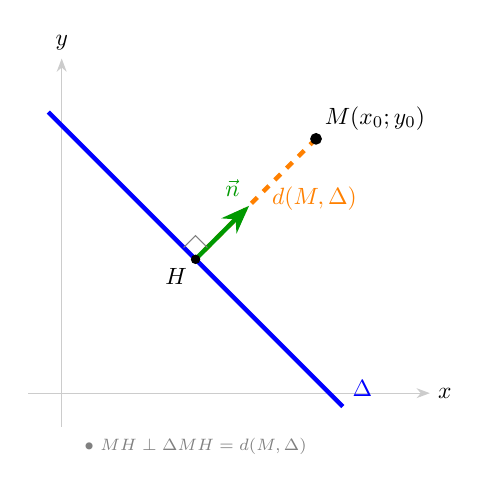
\begin{tikzpicture}[>=Stealth, thick, scale=0.85, every node/.style={scale=0.85}]
                % Trục tọa độ mờ
                \draw[->, gray!40, thin] (-0.5,0) -- (5.5,0) node[right, black] {$x$};
                \draw[->, gray!40, thin] (0,-0.5) -- (0,5.0) node[above, black] {$y$};
                
                % Đường thẳng Delta: x + y - 4 = 0 (Góc -45 độ chuẩn)
                % Vẽ từ (0.2, 3.8) đến (3.8, 0.2)
                \draw[blue, ultra thick] (-0.2, 4.2) -- (4.2, -0.2) node[above right] {$\Delta$};
                
                % Tọa độ các điểm chính xác: M(3.8, 3.8), H(2, 2)
                \coordinate (M) at (3.8, 3.8);
                \coordinate (H) at (2, 2);
                
                % Vẽ đoạn MH (Dashed orange)
                \draw[dashed, orange, ultra thick] (M) -- (H) node[midway, right=0.1cm] {$d(M, \Delta)$};
                
                % Vẽ vector n xuất phát từ H (Cùng phương với HM)
                \draw[->, green!60!black, ultra thick] (H) -- ++(0.8, 0.8) node[above left] {$\vec{n}$};
                
                % Vẽ ký hiệu góc vuông tại H (Xoay 45 độ để khớp với độ dốc -1 của Delta)
                \begin{scope}[shift={(H)}, rotate=45]
                    \draw[gray, thin] (0, 0.25) -- (0.25, 0.25) -- (0.25, 0);
                \end{scope}

                % Các điểm và nhãn
                \filldraw[black] (M) circle (2pt) node[above right] {$M(x_0; y_0)$};
                \filldraw[black] (H) circle (1.5pt) node[below left] {$H$};
                
                % Chú thích ngắn gọn dưới hình
                \node[gray, font=\scriptsize, align=left] at (2.0, -0.8) {$\bullet$ $MH \perp \Delta \implies MH = d(M, \Delta)$};
            \end{tikzpicture}
        \end{column}
    \end{columns}
\end{frame}



\end{document}